\documentclass[10pt,a4paper]{article}
\usepackage[margin=2.1cm]{geometry}
\usepackage[T1]{fontenc}
\usepackage[utf8]{inputenc}
\usepackage{lmodern}
\usepackage{amsmath,amssymb,amsthm}
\usepackage{graphicx}
\usepackage{booktabs}
\usepackage{microtype}
\usepackage[hidelinks,pdfauthor={},pdfcreator={},pdfproducer={}]{hyperref}
\usepackage{url}
\Urlmuskip=0mu plus 1mu
\emergencystretch=2em

\newtheorem{theorem}{Theorem}
\newtheorem{lemma}[theorem]{Lemma}
\newtheorem*{remark}{Remark}
\newcommand{\R}{\mathbb{R}}
\newcommand{\Z}{\mathbb{Z}}

\title{Every non-5-colourable unit-distance graph in the plane\\ has at least 244 edges and at least 51 vertices}
\author{olivierFer3}
\date{November 2026, version 2 \quad (preprint, not reviewed by a human mathematician)}

\begin{document}
\maketitle

\begin{abstract}
We give a computer-assisted proof that every finite unit-distance graph in the Euclidean plane that
is not $5$-colourable has at least $244$ edges and at least $51$ vertices. The previous best bounds in the
literature were $182$ edges and $42$ vertices (de Grey--Parts); version~1 of this note (15 November 2026)
gave $204$ edges and $45$ vertices. The proof combines the averaging argument of Gwyn--Stavrianos with an
explicit periodic $5$-colouring, called ILEP\_S6A, whose fifth colour is a $512$-gon placed near the
midpoints of one hexagon edge out of four, a computer-assisted upper bound
$p_5\le 41149783/10^{10}<1/239$ for its monochromatic unit-segment probability, obtained in exact rational
and ball arithmetic, and the bound $u(50)\le239$ derived from Proposition~12 of \'Agoston--P\'alv\"olgyi.
\end{abstract}

\section{Statement and context}

A \emph{unit-distance graph} is a finite graph whose vertices are points of $\R^2$ and whose edges join
points at distance~$1$. Let $u(n)$ be the maximum number of edges of a unit-distance graph with $n$
vertices.

\begin{theorem}\label{thm:main}
Every finite unit-distance graph in $\R^2$ that is not $5$-colourable has at least $244$ edges and
at least $51$ vertices.
\end{theorem}

In the notation of \cite{dGP}, $e_6\ge244$ and $v_6\ge51$. The statement is unconditional: it says
nothing about the existence of such graphs. These quantities are finite if and only if
$\chi(\R^2)\ge6$. The inequality $\chi(\R^2)\ge6$ has been announced in an OpenAI preprint \cite{OAI},
which we have not checked; that preprint does not concern the bounds proved here.

\paragraph{Versions.} Version~1 of this note (15 November 2026) proved $e_6\ge204$ and $v_6\ge45$ with a
colouring called ILEP256; a simpler colouring, DISQP32, gives $e_6\ge193$ and $v_6\ge44$ and remains the
simple example here. Version~2 keeps the method and changes the colouring: the island of the fifth colour
gets a free centre and free angles, and the hexagons are allowed to become non-convex. Two intermediate
colourings, ILEP\_S5B ($v_6\ge46$) and ILEP\_S5E ($v_6\ge50$), were steps of the optimisation; they are
certified and distributed, but superseded. Version~1 remains available in the repository (tag \texttt{v1}).

\paragraph{Previous work.} Gwyn and Stavrianos \cite{GS} introduced $p_k(c)$, the probability that a
random unit segment is monochromatic for a $k$-colouring $c$ of the plane. They proved that a
non-$k$-colourable unit-distance graph has at least $1/p_k(c)$ edges \cite[Lemma~2.10]{GS}. With four
colours on regular hexagons, and a fifth colour on randomly translated disks
\cite[Lemma~2.23]{GS}, they obtained $e_6\ge180$. De Grey and Parts \cite{dGP} replaced the disks by
the rounded dodecagons of Croft's tiling, of density about $0.229365$ (Croft's ``tortoises''; see
\cite{KMOR} for the construction). They also corrected the rounding of the bounds, using
$e_k\ge\lceil1/p_{k-1}\rceil$ where \cite{GS} had rounded down, and they used the bounds on $u(n)$ of
\cite{AP}. This gave $e_5\ge99$, $v_5\ge28$, $e_6\ge182$ and $v_6\ge42$. Their values of $p_k$ were
computed by numerical integration (Mathematica) and were not certified. Two comments in the
Polymath16 thread \cite{PM16} (28 and 30 June 2022, by the user \texttt{ag24ag24} of the Polymath16 project) are relevant. The first expressed
the hope for ``a more impressive value than 42 using good 5-tilings rather than their Lemma 6''. The
second reported that the hexagonal $5$-tiling tried there was worse and that ``something else is needed there --
I think probably an adaptation of the paper's Lemma 6 taking into account the existence of regions
that cannot contain a vertex of a mono edge''. We found no follow-up in the literature. The present construction is of
this kind: the fifth colour is not translated at random but placed at fixed positions relative to the
hexagons, near edge midpoints, and its shape is optimised together with the hexagons. Related
but different problems include the numerical optimisation of periodic colourings
\cite{Mundinger} and partial proper colourings with voids \cite{Parts}.

\section{The colourings}

Fix rationals $R$ and $s\approx\sqrt3R$, and put $v_1=(3R/2,s/2)$, $v_2=(0,s)$, $c_{ij}=iv_1+jv_2$,
$g_1=2v_1=(3R,s)$ and $g_2=2v_2=(0,2s)$. The colouring is periodic with period lattice
$G=\Z g_1+\Z g_2$, and its period cell $C$ has area $|C|=|\det(g_1,g_2)|$. The hexagons have vertices
$P_0(i,j)=c_{ij}+(R,0)+\delta_0[i\bmod2][j\bmod2]$ and $P_1(i,j)=c_{ij}+(R/2,s/2)+\delta_1[i\bmod2][j\bmod2]$,
with eight rational displacements $\delta$; hexagon $(i,j)$ is
$P_0(i,j)P_1(i,j)P_0(i{-}1,j{+}1)P_1(i{-}1,j)P_0(i{-}1,j)P_1(i,j{-}1)$, and these hexagons tile the plane.
The hexagon $(i,j)$ receives colour $(i\bmod 2)+2(j\bmod 2)\in\{0,1,2,3\}$, as in \cite[Fig.~6]{GS}.
Colour~$4$ is an ``island'' $E$ and its $G$-translates. $E$ is the polygon $W_0W_1\cdots W_{n-1}$ with
$W_k=m+\rho_k(\cos\psi_k,\sin\psi_k)$, the offsets being rounded to $10^{-12}$; it lies near the midpoint of the
horizontal edge shared by the hexagons $(0,0)$ and $(0,1)$, so the fifth colour covers one horizontal edge
out of four.

\paragraph{ILEP\_S6A (presented).} $R=140120428967/(2.5\cdot10^{11})\approx0.56048$ and
$s=970782808597/10^{12}$, so that $|C|\approx3.26464$. The island has $n=512$ vertices; its centre $m$ and its
angles $\psi_k$ are free parameters of the optimisation. The displacements are large ($|\delta|\le0.31$): the
hexagons of colours $0$ and $2$ are sheared until each of them has one reflex vertex, with turning
determinants $-0.063$ and $-0.065$. Both reflex vertices lie strictly inside a sector of the island, so the
non-convex part is entirely removed by the fifth colour. The hexagons of colours $1$ and $3$ remain strictly
convex. The colour regions have areas $0.604$, $0.721$, $0.603$, $0.721$ and $0.615$ (colours $0$--$4$), and
diameters $1.145$, $1.116$, $1.145$, $1.121$ and $1.320$. The island is star-shaped with respect to $m$ but
not convex; its boundary is irregular (Figure~\ref{fig}). These numbers only describe the construction: the
certified object is the colouring defined by the rational coordinates of the JSON file (see \emph{Exact
definition} below).

\paragraph{DISQP32 (simple example).} The hexagons are regular, up to the rounding of $s$, with $R=28360517/(5\cdot10^7)$.
$E$ is a rational $32$-gon of circumradius $0.48498$ centred at $(0,\,122773743/(2.5\cdot10^8))$.

\paragraph{Other colourings of the repository.} ILEP256 (version~1) has slightly deformed hexagons
($|\delta|\le0.0068$) and a $256$-vertex island centred at the midpoint of $P_1(0,0)P_0(-1,1)$ with
$\psi_k=2\pi k/256$. ILEP\_S5B ($256$ vertices) and ILEP\_S5E ($512$ vertices) are intermediate steps between
ILEP256 and ILEP\_S6A, with convex hexagons. ILEP\_S7\_93 is a variant of ILEP\_S6A whose island was
simplified to $93$ vertices (Section~\ref{sec:checks}).

\paragraph{Exact definition.} The certified colourings are the \emph{exact rational} colourings
defined by the files \texttt{<label>\_config.json}. These files list $g_1$, $g_2$ and a family of closed
convex polygons $P_1,\dots,P_N$ with rational vertices, each with a colour ($N=523$ for ILEP\_S6A and $52$
for DISQP32). The pieces are the hexagons minus the fifth-colour regions, cut into convex pieces, together
with convex sectors of $E$. They are rational variants of the floating-point colourings found by
optimisation. Because the argument applies to any measurable periodic colouring, the bound concerns exactly
these files. A point $x$ receives the colour of the piece of smallest index $i$ with $x\in P_i+G$. This rule is
$G$-periodic and Borel. Boundaries form a null set, so the rule does not affect $p_5$.

\begin{figure}[t]
\centering
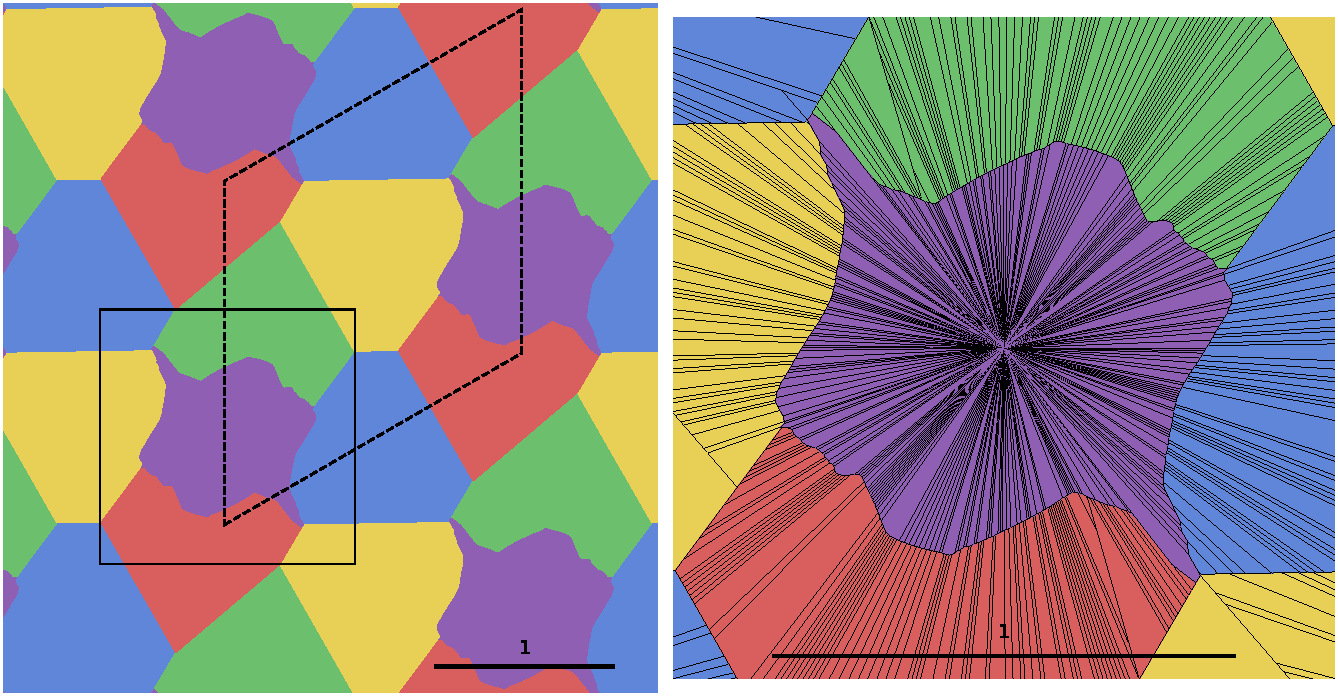
\includegraphics[width=0.98\textwidth]{fig_s6a.pdf}
\caption{Left: ILEP\_S6A around one period cell (dashed parallelogram spanned by $g_1,g_2$). Red, blue, green,
yellow: colours $0$--$3$ on the deformed hexagons; the red and green hexagons (colours $0$ and $2$) are
sheared, and their reflex vertices are hidden under the islands. Purple: colour $4$ (the island). Right: zoom
on the framed island, with the boundaries of the $523$ convex pieces of the certified colouring (and of their
translates). The bars have length $1$.}
\label{fig}
\end{figure}

\section{From \texorpdfstring{$p_5$}{p5} to edges and vertices}

For a $G$-periodic Borel colouring $c$, let $u(\theta)=(\cos\theta,\sin\theta)$ and
\[
p(c)=\frac{1}{2\pi|C|}\int_0^{2\pi}\bigl|\{x\in C:\ c(x)=c(x+u(\theta))\}\bigr|\,d\theta .
\]

\begin{lemma}[{\cite[Lemma~2.10]{GS}, periodic case}]\label{lem:gs}
If a finite unit-distance graph $H$ is not $k$-colourable and $c$ is a $G$-periodic Borel
$k$-colouring, then $|E(H)|\ge 1/p(c)$.
\end{lemma}
\begin{proof}
Draw $x$ uniformly in $\R^2/G$ and a rotation $\rho_\theta$ with $\theta$ uniform, and map $H$ by
$v\mapsto x+\rho_\theta v$. For each edge $vw$, the image of $v$ is uniform on $\R^2/G$ and
independent of the direction of $vw$, which is uniform. So the edge is monochromatic with
probability $p(c)$ (Fubini). The image of $H$ always has a monochromatic edge, so
$1\le\mathbb E[\#\text{mono}]=|E(H)|\,p(c)$.
\end{proof}

The same argument fits the framework of \cite{GS}, which uses Jordan measure. The set
$S=\{(x,\theta)\in C\times[0,2\pi]:c(x)=c(x+u(\theta))\}$ is Jordan-measurable in $\R^3$. Indeed, let
$Z$ be the union of the boundaries of the translates $P_i+g$. Two closed convex pieces with disjoint
interiors cannot meet the interior of each other, so $c$ is locally constant outside $Z$. Hence
$\partial S$ is contained in the union of $\partial(C\times[0,2\pi])$, of $\{(x,\theta):x\in Z\}$ and of
$\{(x,\theta):x+u(\theta)\in Z\}$, restricted to the compact set $\overline C\times[0,2\pi]$. Only
finitely many edges of $Z$ meet the bounded set $\overline C+\overline{B}(0,1)$. For each such edge
$z:[0,1]\to\R^2$, the corresponding parts of these two sets are the images of the two-dimensional set
$[0,1]\times[0,2\pi]$ under the Lipschitz maps $(t,\theta)\mapsto(z(t),\theta)$ and
$(t,\theta)\mapsto(z(t)-u(\theta),\theta)$. They therefore have three-dimensional measure zero, and so
does $\partial(C\times[0,2\pi])$. Thus $\partial S$ is a null set. By Lemma~\ref{lem:gs} and
Theorem~\ref{thm:cert} below, a non-$5$-colourable graph has more than $10^{10}/41149783>243.01$ edges,
hence at least $244$. DISQP32 gives at least $193$.

\paragraph{Vertices.} \'Agoston and P\'alv\"olgyi \cite[Prop.~12]{AP} state, for an \emph{extremal}
unit-distance graph $G$ with $n$ vertices and $m=u(n)$ edges, the inequality
$n^2-n\ge 4m-12n+24+\sum_v\binom{\deg v}{2}$. Its proof uses the construction of their Section~3:
unit circles around the vertices are cut into $2m$ arcs by the points of $G$. This requires every
vertex to have degree at least $3$, so that at least three points lie on each circle and every pair
of points is joined by at most two arcs. Extremality ensures that any two points at unit distance are
adjacent. We apply it only to an extremal graph $G$. If all degrees of $G$ are at least $3$, the
inequality holds. Otherwise, deleting a vertex of degree at most $2$ gives $u(n)\le u(n-1)+2$, as
noted in \cite[note~6, p.~12]{AP}. The sum is at least
$J(n,2m)=(n-r)\binom{q}{2}+r\binom{q+1}{2}$, where $2m=qn+r$ with $0\le r<n$. Let $P(n)$ be the
largest $m$ with $n^2-n\ge 4m-12n+24+J(n,2m)$ (the right-hand side is increasing in $m$). We start from
$u(22)\le61$ \cite{AMP} and also use Schade's lemma $u(n)\le\lfloor n\,u(n-1)/(n-2)\rfloor$
\cite[Lemma~2]{AMP}. Hence $u(n)\le B(n)$ with $B(22)=61$ and
\[
B(n)=\min\Bigl(\Bigl\lfloor \frac{n\,B(n-1)}{n-2}\Bigr\rfloor,\ \max\bigl(P(n),\,B(n-1)+2\bigr)\Bigr)\qquad(n\ge23).
\]
Schade's lemma is at least as good for $n\le32$, Proposition~12 is better for $n\ge33$. In exact integer arithmetic
(\texttt{verifier/u\_bounds.py}) the complete chain is
\[
\begin{array}{c|ccccccccccccccc}
n & 22 & 23 & 24 & 25 & 26 & 27 & 28 & 29 & 30 & 31 & 32 & 33 & 34 & 35 & 36\\ \hline
B(n) & 61 & 66 & 72 & 78 & 84 & 90 & 96 & 103 & 110 & 117 & 124 & 130 & 136 & 142 & 148
\end{array}
\]
\[
\begin{array}{c|cccccccccccccc}
n & 37 & 38 & 39 & 40 & 41 & 42 & 43 & 44 & 45 & 46 & 47 & 48 & 49 & 50\\ \hline
B(n) & 154 & 160 & 166 & 172 & 179 & 185 & 192 & 198 & 205 & 212 & 218 & 225 & 232 & 239
\end{array}
\]
For $22\le n\le30$ these are the values of \cite[Thm.~1(b)]{AMP}, and for $32\le n\le50$ they coincide with the
list of upper bounds given by de Grey and Parts \cite[note~3]{dGP}, which reads
``\dots, 185, 192, 198, 205, 212, 218, 225, 232, 239, 246, 254, \dots'' for $n=42,\dots,52$.
The last steps are detailed in Table~\ref{tab:u}.

\begin{table}[ht]
\centering
\begin{tabular}{rrrrrrr}
\toprule
$n$ & $\lfloor\frac{nB(n-1)}{n-2}\rfloor$ & $\max(P(n),B(n-1){+}2)$ & $B(n)$ & $n^2-n$ & RHS$(B(n))$ & RHS$(B(n){+}1)$\\
\midrule
45 & 207 & 205 & 205 & 1980 & 1969 & 1991\\
46 & 214 & 212 & 212 & 2070 & 2066 & 2088\\
47 & 221 & 218 & 218 & 2162 & 2141 & 2163\\
48 & 227 & 225 & 225 & 2256 & 2238 & 2260\\
49 & 234 & 232 & 232 & 2352 & 2335 & 2357\\
50 & 241 & 239 & 239 & 2450 & 2432 & 2454\\
\bottomrule
\end{tabular}
\caption{The bounds $u(n)\le B(n)$ for $45\le n\le 50$. Second column: Schade's bound; RHS$(m)=4m-12n+24+J(n,2m)$. In each row $P(n)=B(n)$:
the right-hand side is $\le n^2-n$ at $m=B(n)$ and $>n^2-n$ at $m=B(n)+1$.}
\label{tab:u}
\end{table}

Since $u$ is non-decreasing, a graph with at most $50$ vertices has at most $239<244$ edges. Therefore
$v_6\ge51$. (DISQP32 gives $v_6\ge44$ because $u(43)\le192<193$; ILEP\_S5B and ILEP\_S5E give $v_6\ge46$ and
$v_6\ge50$, from $e_6\ge208>205\ge u(45)$ and $e_6\ge235>232\ge u(49)$.) The next threshold would be
$p_5<1/246$, since $u(51)\le246$.

\section{Certification of \texorpdfstring{$p_5$}{p5}}

\begin{theorem}\label{thm:cert}
For the exact colourings defined by the JSON files,
\[
p(\mathrm{ILEP\_S6A})\le 41149783/10^{10}<1/239
\qquad\text{and}\qquad
p(\mathrm{DISQP32})\le 51864759/10^{10}<1/192 .
\]
Moreover $p(\mathrm{ILEP256})\le 24616771/(5\cdot10^9)<1/203$ (version~1),
$p(\mathrm{ILEP\_S5B})\le24135541/(5\cdot10^9)<1/205$, $p(\mathrm{ILEP\_S5E})\le42565529/10^{10}<1/232$ and
$p(\mathrm{ILEP\_S7\_93})\le5137931/(1.25\cdot10^9)<1/239$.
\end{theorem}

The final comparisons are exact: $41149783\cdot239=9834798137<10^{10}$ and $51864759\cdot192=9958033728<10^{10}$.
The bound for ILEP\_S6A does not reach $1/246$: $41149783\cdot246=10122846618>10^{10}$. The floating-point
values are $p(\mathrm{ILEP\_S6A})\approx0.0041078$ and $p(\mathrm{DISQP32})\approx0.0051253$.

\paragraph{1. Exact tiling.} In rational arithmetic we check: (i) each piece is strictly
convex and counter-clockwise. This means all turns are positive \emph{and} the piece equals its
convex hull, a test that rejects star polygons. It holds for 523/523 pieces of ILEP\_S6A. (ii) The areas
of the pieces sum to $|C|$ exactly. (iii) Every pair $P_i$, $P_j+g$ with $(j,g)\ne(i,0)$ whose
bounding disks meet has an intersection of area~$0$; the list of translations tested is complete, since
$|a|\,|C|\le|t|\,|g_2|$ for $t=ag_1+bg_2$, and similarly for $b$. For ILEP\_S6A, $78897$ pairs are tested.
Facts (i)--(iii) imply that the $G$-translates of the pieces tile the plane (Lemma~\ref{lem:tiling}).

\begin{lemma}\label{lem:tiling}
Let $P_1,\dots,P_N$ be compact convex polygons with $\sum_i|P_i|=|C|$ such that the interiors of $P_i+g$ and
$P_j+h$ are disjoint for $(i,g)\ne(j,h)$ in $\{1,\dots,N\}\times G$. Then the translates $P_i+g$ cover $\R^2$.
\end{lemma}
\begin{proof}
Let $\pi:\R^2\to T=\R^2/G$ and let $\mu$ be the Haar measure of $T$, of mass $|C|$. Boundaries of convex
polygons are null sets and $\pi$ is injective on the disjoint union of the interiors, so
$\mu(\pi(\bigcup P_i))=\sum|P_i|=|C|$. Hence $U=\bigcup_{i,g}(P_i+g)=\pi^{-1}(\pi(\bigcup P_i))$ has a null
complement. $U$ is closed, as a locally finite union of compact sets, so $\R^2\setminus U$ is an open null set,
hence empty.
\end{proof}

This lemma uses only the list of pieces, not the way it was produced. In ILEP\_S6A the hexagons of colours $0$
and $2$ are not convex; the construction splits each of them into a fan of triangles from its reflex vertex,
merged into convex parts, before removing the islands. We do not prove that this splitting is correct in
general, and we do not need to: a wrong splitting could only make (i), (ii) or (iii) fail, or produce another
colouring, which would then be valid and certified for what it is. For ILEP\_S6A, an independent exact check
(by another splitting of the hexagons) confirms that the pieces of colour $c<4$ form exactly the hexagon of
colour $c$ minus the islands. The completeness of the pairs in step~2 below is a separate check.

\paragraph{2. Reduction to areas.} Let $A_{PQ}(u)=|P\cap(Q-u)|$. Using the symmetry
$p(\theta+\pi)=p(\theta)$, and no other symmetry, we get
\[ p(c)=\frac{1}{\pi|C|}\int_0^\pi\sum_{(P,Q)}A_{PQ}(u(\theta))\,d\theta, \]
where $P$ ranges over the pieces and $Q$ over the translates of pieces of the same colour.
Pairs of colour $4$ are included. A pair can contribute only if $\operatorname{dist}(0,Q-P)<1<
\max|{\rm vertex}(Q-P)|$, which leaves $4754$ pairs for ILEP\_S6A and $394$ for DISQP32. The enumeration of
translations is complete: the translations are bounded from a computed radius of the pieces
(here $|a|,|b|\le3$), and the second verifier checks independently that $|a|\ge2$ or $|b|\ge2$ puts every
pair of pieces at distance $>1$. On each box of angles we also discard the pairs whose angular sector misses
the box. The sector is enclosed rigorously using ball arithmetic.

\paragraph{3. Bound on a box $I=[x_0\pi,x_1\pi]$.} (M1) By Brunn--Minkowski, the function $u\mapsto\sqrt{A_{PQ}(u)}$ (as a function of the translation
vector $u\in\R^2$, not of $\theta$) is concave on the support $\operatorname{int}(Q-P)$ of $A_{PQ}$.
Let $u_0$ be a rational point with $A_0=A_{PQ}(u_0)>0$ at which $A_{PQ}$ is differentiable, with
gradient $\nabla$; only this anchor point needs to be a point of differentiability. Put $d=u-u_0$
and $T=\sqrt{A_0}+\nabla\cdot d/(2\sqrt{A_0})$, the tangent of $\sqrt{A_{PQ}}$ at $u_0$. Concavity gives
$\sqrt{A_{PQ}(u)}\le T$ on the support, and $T\ge\sqrt{A_{PQ}(u)}\ge0$ there. Hence
$A_{PQ}(u)\le T^2=A_0+\nabla\cdot d+(\nabla\cdot d)^2/(4A_0)$. Outside the support, $A_{PQ}(u)=0\le T^2$.
So the bound holds for \emph{all} $u$. The gradient is exact: translating $Q-u_0$ by $-d$ moves only the edges $f$ of $Q-u_0$,
so $\nabla=-\sum_f n_f\,|f\cap P|$, with outer normals $n_f$. In the code, $P\cap(Q-u_0)$ is computed by
Sutherland--Hodgman clipping of $P$ by the half-planes of $Q-u_0$, and each edge of the intersection is
labelled as carried by $\partial P$ or by an edge of $Q-u_0$. Since the vectors (outer normal)$\times$(length)
of the edges of a closed polygon sum to zero, $\nabla=\sum_e n_e\,|e|$ over the edges $e$ of the
intersection labelled as carried by $\partial P$; this is the sum the code evaluates. Differentiability holds when no edge of $P$ is collinear with an edge of $Q-u_0$, which is
checked exactly. The right-hand side is a quadratic
polynomial in $(\cos\theta,\sin\theta)$ with rational coefficients, and its integral over $I$ is
evaluated from closed-form moments in ball arithmetic (Arb via python-flint, \cite{flint}). (M2) If
a rational rectangle $K$ contains the arc $u(I)$, then $A_{PQ}(u(\theta))\le|P\cap(Q\oplus(-K))|$ on
$I$. For each pair, either bound may be used; floating-point numbers only \emph{choose} $u_0$, the
bound and the boxes, so they never enter the validity. The box bounds are summed exactly. The total is
divided by $\pi|C|$ in ball arithmetic and rounded up. We use $1024$ boxes for ILEP\_S6A (about $10$ minutes
on a laptop with three processes) and $256$ for DISQP32.

\section{Checks}\label{sec:checks}

All the checks below were designed and run by AI agents (see \emph{Use of AI} below). \textbf{No human has reviewed
the certificates, the code or the proofs.}

\paragraph{The certificate.} The rigorous bound rests on the certifier alone: exact rational arithmetic for
the geometry and the sums, and Arb ball arithmetic for the box integrals and for $\pi$. A separate program of
the certifier's package recomputes every box bound from the JSON files; it uses the same library, so it is a
recomputation, not an independent proof.

\paragraph{Two verifiers.} A second verifier, which does not import the certifier and does not use
python-flint, checks exactly, in Python \texttt{Fraction} arithmetic, the tiling (convexity, areas, disjoint
interiors), the completeness of the translations, the list of contributing pairs and the rational additions of
the box bounds, including the final comparison with $\pi>314159265358979/10^{14}$. It does \emph{not}
recertify the box bounds in interval arithmetic. It also recomputes every box integral in floating point
(GEOS areas, explicit breakpoints, Gauss--Legendre); this numerical check ``N'' is not a proof. For
ILEP\_S6A all exact checks pass, every certified box bound exceeds the floating-point integral, by at least
$5.7\cdot10^{-10}$, and the recomputed value is $p\approx0.0041078$. In addition, the \emph{unmodified}
verifier and recomputation program of version~1 were run on ILEP\_S5B, ILEP\_S5E, ILEP\_S6A and
ILEP\_S7\_93: all exact checks pass and every box bound is confirmed. For ILEP\_S5B and ILEP\_S5E the set of
pairs of the certifier was compared with that of the verifier and found exactly equal.

\paragraph{Monte Carlo.} A Monte Carlo program, written from scratch and importing no code of the project,
draws $4\cdot10^7$ random unit segments per colouring and reads only the JSON file. It gives
$0.0041071\pm1.0\cdot10^{-5}$ for ILEP\_S6A ($-0.8\sigma$ from the certified bound),
$0.0041073\pm1.0\cdot10^{-5}$ for ILEP\_S7\_93, $0.0048140\pm1.1\cdot10^{-5}$ for ILEP\_S5B,
$0.0042476\pm1.0\cdot10^{-5}$ for ILEP\_S5E and, as a control, $0.0049223\pm1.1\cdot10^{-5}$ for ILEP256
(floating-point value $0.0049197$). No point is uncovered or doubly covered. With $\sigma\approx10^{-5}$ this
check would detect only an error of about $3\cdot10^{-5}$ or more; it is independent of the certifier's code,
not of the AI that wrote both. The program and its results are in the repository.

\paragraph{Reviews of the modifications.} The modifications of the certifier for version~2 (free centre and
angles of the island, input directory, splitting of non-convex hexagons) are confined to the construction of
the colouring; the modules performing the exact checks, the pair enumeration and the box bounds are
byte-identical to version~1. They were reviewed by an AI agent that had not written them, and the splitting of
the hexagons and its output for ILEP\_S6A were reviewed by another one, with an exact check by an independent
splitting. Neither review found a decisive problem; both note that the fan splitting is not proved correct in
general, which does not affect the validity (Lemma~\ref{lem:tiling}).

\paragraph{The variant ILEP\_S7\_93.} This variant has a $93$-vertex island and $104$ pieces and a better bound
($5137931/(1.25\cdot10^9)\approx0.0041103$), but crosses no new threshold. It passes the certifier, the exact
checks of both verifiers, the recomputation and the Monte Carlo check. The numerical check N fails on two of the
$1024$ boxes: there the certified bound exceeds the floating-point integral by only about $3\cdot10^{-21}$
(relative margin $2.6\cdot10^{-14}$ and $3.1\cdot10^{-14}$), less than the absolute floor $10^{-16}$ of the error
estimate of N. No box bound is below the integral, and Gauss--Legendre rules with $10$, $20$ and $30$ nodes
differ by at most $4\cdot10^{-22}$ there, $7$ to $60$ times less than the margin. The alert reflects an almost
exact enclosure, not a missing contribution; since N is not lifted by the verifier itself, we present ILEP\_S6A.

\begin{remark}[heuristic: where the gain comes from]
The following is an empirical observation, not a proof. The optimisation from ILEP256 to ILEP\_S6A shears the
hexagons of colours $0$ and $2$ into elongated oblique shapes, enlarges them (area $0.540\to0.604$) and shrinks
the hexagons of colours $1$ and $3$ (area $0.791\to0.721$), while the island becomes longer and its boundary
irregular. A Monte Carlo decomposition for the intermediate colouring ILEP\_S5E ($10^7$ segments) shows that the
contribution of segments with both end points in the same hexagon drops by about $29\,\%$ with respect to
ILEP256 (from $3.54\cdot10^{-3}$ to $2.52\cdot10^{-3}$), partly offset by the island, which now contains unit
chords ($0.11\cdot10^{-3}\to0.46\cdot10^{-3}$), and by pairs of neighbouring regions. All the regions have
a diameter only slightly above $1$ ($1.12$--$1.15$ for the hexagons of ILEP\_S6A). A plausible explanation is
that the measure of the unit segments inside such a region depends very non-linearly on the excess of its
diameter over $1$ and on the shape of opposite corners, so that small deformations remove many interior unit
segments.
\end{remark}

\section{Limitations and remarks}

\begin{itemize}
\item \textbf{No human review.} The certificates, the proofs, the code and its modifications have been checked
only by AI agents, which may share blind spots. The proof rests on the inclusion principle of Arb, which is
standard and documented.
\item \textbf{Novelty.} To our knowledge, bounds beyond $e_6\ge182$ and $v_6\ge42$ have not appeared in the
literature apart from version~1 of this note. Our search covered arXiv, the tables of contents of
Geombinatorics 2022--2026, the Polymath16 threads and general web search. It is not exhaustive: we could not
read the full text of recent Geombinatorics issues, nor use Google Scholar.
\item \textbf{$\chi(\R^2)\ge6$} is not established independently here. Theorem~\ref{thm:main} holds in
any case.
\item \textbf{$v_6\ge52$} would require $p_5<1/246\approx0.0040650$, about $1.3\,\%$ below the bound of
ILEP\_S6A. Within the present family of colourings the optimisation has converged near $p_5\approx0.0041075$;
a richer family would be needed.
\end{itemize}

\begin{remark}[$v_5\ge29$]
From $e_5\ge99$ \cite{dGP} and $u(28)\le96$ \cite[Thm.~1(b)]{AMP}, it follows that every
non-$4$-colourable unit-distance graph has at least $29$ vertices. This remark uses only the published
bounds of \cite{dGP} and \cite{AMP}. As a secondary computation, not audited and not part of the
results of this note, the same certifier applied to the four-colour hexagon tiling with $D=1.133523$
gives $p_4\le101531397/10^{10}<1/98$, consistent with $e_5\ge99$.
\end{remark}

\paragraph{Use of AI.} The construction, the optimisation of the colourings, the certification
code and its modifications, the proofs and this note were produced with Claude Code (Anthropic). Further AI
agents (Claude) wrote the Monte Carlo program, reviewed the modifications of the certifier and the splitting
of the hexagons, and ran the verifiers. For version~1, ChatGPT (OpenAI) also performed cross-checks:
literature search, a reading of the arguments and execution of the verifiers. These checks are separate
programs and separate agents, but they are all AI-assisted and may share blind spots; no human mathematician
has reviewed this work. Code, certificates, logs and the Monte Carlo program: see the accompanying repository
(\texttt{README.md}).

\begin{thebibliography}{9}\small
\bibitem{AMP} B.~Alexeev, D.~G.~Mixon, H.~Parshall, \emph{The Erd\H{o}s unit distance problem for small
point sets}, arXiv:2412.11914v2 (2025).
\bibitem{AP} P.~\'Agoston, D.~P\'alv\"olgyi, \emph{An improved constant factor for the unit distance
problem}, arXiv:2006.06285v3 (2021); Studia Sci.\ Math.\ Hungar.\ 59 (2022) 40--57.
\bibitem{dGP} A.~D.~N.~J.~de Grey, J.~Parts, \emph{On lower bounds of the order of $k$-chromatic unit
distance graphs}, arXiv:2303.14714v1 (2023); Geombinatorics 32(2) (2022), 72.
\bibitem{flint} FLINT/Arb documentation, \url{https://flintlib.org/doc/arb/index.html}; python-flint 0.9.0.
\bibitem{GS} H.~Gwyn, J.~Stavrianos, \emph{A finite graph approach to the probabilistic
Hadwiger--Nelson problem}, arXiv:2008.07987v1 (2020); Geombinatorics 32(1) (2022), 5.
\bibitem{KMOR} T.~Keleti, M.~Matolcsi, F.~M.~de Oliveira Filho, I.~Z.~Ruzsa, \emph{Better bounds for planar
sets avoiding unit distances}, Discrete Comput.\ Geom.\ 55 (2016) 642--661; arXiv:1501.00168v2.
\bibitem{Mundinger} K.~Mundinger, M.~Zimmer, A.~Kiem, C.~Spiegel, S.~Pokutta, \emph{Neural discovery in
mathematics: do machines dream of colored planes?}, arXiv:2501.18527v3 (ICML 2025).
\bibitem{OAI} OpenAI, \emph{The Euclidean plane is not five-colorable}, preprint (23 Sept.\ 2026),
\url{https://github.com/openai/math}.
\bibitem{Parts} J.~Parts, \emph{What percent of the plane can be properly 5- and 6-colored?},
arXiv:2010.12668; Geombinatorics 30(1).
\bibitem{PM16} D.~G.~Mixon (blog), \emph{Polymath16, seventeenth thread: declaring victory}, comments of
28 June 2022 (6:58 pm) and 30 June 2022 (12:22 am) by \texttt{ag24ag24},
\url{https://dustingmixon.wordpress.com/2021/02/01/polymath16-seventeenth-thread-declaring-victory/}.
\end{thebibliography}
\end{document}
